\chapter{队列}

\section{队列}

\subsection{队列(Queue)}

队列是一种运算受限的线性数据结构,不同于栈的先进后出(FILO),队列中的元素只能先进先出(FIFO, First In First Out)。\\

队列的出口端叫作队头(front),队列的入口端叫作队尾(rear)。队列只允许在队尾进行入队(enqueue),在队头进行出队(dequeue)。\\

与栈类似,队列既可以用数组来实现,也可以用链表来实现。其中用数组实现时,为了入队操作的方便,把队尾位置规定为最后入队元素的下一个位置。\\

\subsection{入列(enqueue)}

入队就是把新元素放入队列中,只允许在队尾的位置放入元素,新元素的下一个位置将会成为新的队尾。入队操作的时间复杂度是$ O(1) $。

\begin{figure}[H]
	\centering
	\begin{tikzpicture}
		\fill[green!20] (5.1,.35) rectangle (-.6,-.35);
		\draw[green,thick] (-.6,.35) -- (5.1,.35) |- (-.6,-.35);
		\foreach \i/\name in {0/A,1/B,2/C}
		\node[queue element] (\name) at (1.5*\i,0) {\name};
		\draw[<-] ([yshift=.2cm]C.north) -- ++ (0,.5) node[above] {rear};
		\draw[<-] ([yshift=.2cm]A.north) -- ++ (0,.5) node[above] {front};
		\path (6,0) node[right] {before};
		\node[queue element] (D) at (6,1) {D};
		\draw[<-,very thick] (4.7,0) to[out=0,in=180] (D.south);

		\scope[yshift=-3cm]
		\fill[green!20] (5.1,.35) rectangle (-.6,-.35);
		\draw[green,thick] (-.6,.35) -- (5.1,.35) |- (-.6,-.35);
		\foreach \i/\name in {0/A,1/B,2/C,3/D}
		\node[queue element] (\name) at (1.5*\i,0) {\name};
		\draw[<-] ([yshift=.2cm]D.north) -- ++ (0,.5) node[above] {rear};
		\draw[<-] ([yshift=.2cm]A.north) -- ++ (0,.5) node[above] {front};
		\path (6,0) node[right] {after};
		\endscope
	\end{tikzpicture}
	\caption{入队}
\end{figure}

\vspace{0.5cm}

\subsection{出队(dequeue)}

出队就是把元素移出队列,只允许在队头一侧移出元素,出队元素的后一个元素将成为新的队头。出队操作的时间复杂度是$ O(1) $。

\begin{figure}[H]
	\centering
	\begin{tikzpicture}
		\fill[green!20] (5.1,.35) rectangle (-.6,-.35);
		\draw[green,thick] (-.6,.35) -- (5.1,.35) |- (-.6,-.35);
		\foreach \i/\name in {0/A,1/B,2/C,3/D}
		\node[queue element] (\name) at (1.5*\i,0) {\name};
		\draw[<-] ([yshift=.2cm]D.north) -- ++ (0,.5) node[above] {rear};
		\draw[<-] ([yshift=.2cm]A.north) -- ++ (0,.5) node[above] {front};
		\draw[->,very thick] (-.7,0) to[out=180,in=90] ++ (-1,-1);
		\path (6,0) node[right] {before};

		\scope[yshift=-3cm]
		\fill[green!20] (5.1,.35) rectangle (-.6,-.35);
		\draw[green,thick] (-.6,.35) -- (5.1,.35) |- (-.6,-.35);
		\foreach \i/\name in {1/B,2/C,3/D}
		\node[queue element] (\name) at (1.5*\i,0) {\name};
		\draw[<-] ([yshift=.2cm]D.north) -- ++ (0,.5) node[above] {rear};
		\draw[<-] ([yshift=.2cm]B.north) -- ++ (0,.5) node[above] {front};
		\path (6,0) node[right] {after};
		\endscope
	\end{tikzpicture}
	\caption{出队}
\end{figure}

\newpage

\section{循环队列}

\subsection{循环队列(Circular Queue)}

如果不断出队,队头左边的空间就失去了作用,那队列的容量就会变得越来越小。

\begin{figure}[H]
	\centering
	\begin{tikzpicture}
		\fill[green!20] (8.1,.35) rectangle (-.6,-.35);
		\draw[green,thick] (-.6,.35) -- (8.1,.35) |- (-.6,-.35);
		\foreach \i/\name in {0/A,1/B,2/C,3/D,4/E,5/F}
		\node[queue element] (\name) at (1.5*\i,0) {\name};
		\draw[<-] ([yshift=.2cm]F.north) -- ++ (0,.5) node[above] {rear};
		\draw[<-] ([yshift=.2cm]D.north) -- ++ (0,.5) node[above] {front};
		\draw[->,very thick] (-.7,0) to[out=180,in=90] ++ (-1,-1);

		\draw[-, red] (-0.5,0.5) -- (0.5,-0.5);
		\draw[-, red] (1,0.5) -- (2,-0.5);
		\draw[-, red] (2.5,0.5) -- (3.5,-0.5);
	\end{tikzpicture}
	\caption{队列存在的问题}
\end{figure}

用数组实现的队列可以采用循环队列的方式来维持队列容量的恒定。为充分利用空间,克服假溢出的现象,在数组不做扩容的情况下,将队列想象为一个首尾相接的圆环,可以利用已出队元素留下的空间,让队尾指针重新指回数组的首位。这样一来整个队列的元素就循环起来了。

\begin{figure}[H]
	\centering
	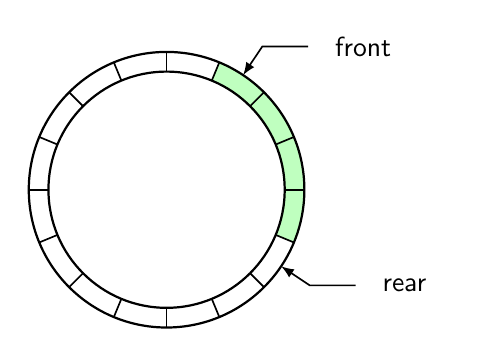
\begin{tikzpicture}[>=latex,font=\sffamily,semithick,scale=1.75]
		\fill [green!25] (0,0) -- (67.5:1) arc [end angle=-22.5, start angle=67.5, radius=1] -- cycle;
		\draw [thick] (0,0) circle (1);
		\foreach \angle in {90,67.5,...,-67.5}
		\draw (\angle:1) -- (\angle-180:1);
		\node [circle,thick,fill=white,draw=black,align=center,minimum size=3cm] at (0,0) {};
		\draw [<-] (56.25:1) -- (56.25:1.25) -- +(.333,0)
		node [right,inner xsep=.333cm] (front) {front};
		\draw [<-] (-33.75:1) -- (-33.75:1.25) -- +(.333,0)
		node [right,inner xsep=.333cm] (rear) {rear};
	\end{tikzpicture}
	\caption{循环队列}
\end{figure}

在物理存储上,队尾的位置也可以在队头之前。当再有元素入队时,将其放入数组的首位,队尾指针继续后移即可。队头和队尾互相追赶,这个追赶的过程就是入队的出队的过程。\\

如果队尾追上队头说明队列满了,如果队头追上队尾说明队列为空。循环队列并非真正地把数组弯曲,利用求余操作就能使队头和队尾指针不会跑出数组的范围,逻辑上实现了弯曲的效果。\\

假设数组的最大容量为MAX:

\begin{itemize}
	\item 入队时队尾指针后移:(rear + 1) \% MAX

	\item 出队时队头指针后移:(front + 1) \% MAX

	\item 判断队满:(rear + 1) \% MAX == front

	\item 判断队空:front == rear
\end{itemize}

需要注意的是,队尾指针指向的位置永远空出一位,所以队列最大容量比数组长度小1。\\

\mybox{入队}

\begin{lstlisting}[language=C]
void enqueue(Queue *queue, dataType val) {
    queue->data[queue->rear] = val;
    queue->rear = (queue->rear + 1) % queue->max;
}
\end{lstlisting}

\vspace{0.5cm}

\mybox{出队}

\begin{lstlisting}[language=C]
dataType dequeue(Queue *queue) {
    dataType ret = queue->data[queue->front];
    queue->front = (queue->front + 1) % queue->max;
    return ret;
}
\end{lstlisting}

\newpage

\section{栈实现队列}

\subsection{栈实现队列}

栈是特性是FILO,而队列是FIFO,因此可以使用两个栈来实现队列的效果。\\

可以将一个栈当作输入栈,用于push()数据,另一个栈当作输出栈,用于pop()和peek()数据。每次pop()或peek()时,若输出栈为空则将输入栈的全部数据依次弹出并压入输出栈,这样输出栈从栈顶往栈底的顺序就是队列从队首往队尾的顺序。\\

用两个栈来实现队列的情况在生活中也经常出现。去医院挂号等待,等待的时候把病历给护士, 护士面前放了两堆病历。等着无聊就看护士是怎么管理病历的。发现一个堆是倒着放的,一个堆是正着放的。新过来的病人把病历给她时,她就把病历倒着放到第一堆,有病人看病结束后,从第二堆的开头翻一个新的病历,然后叫病人。如果第二堆没了话,就直接把第一堆翻过来放到第二推上面。

\begin{figure}[H]
	\centering
	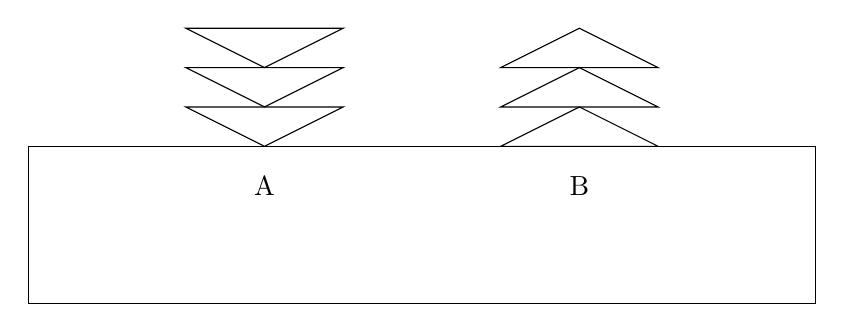
\begin{tikzpicture}
		\draw[-] (0,0) rectangle (10,2);
		\draw (3,1.5) node{A};
		\draw (7,1.5) node{B};

		\draw[-] (2,2.5) -- (4,2.5) -- (3,2) -- cycle;
		\draw[-] (2,3) -- (4,3) -- (3,2.5) -- cycle;
		\draw[-] (2,3.5) -- (4,3.5) -- (3,3) -- cycle;

		\draw[-] (6,2) -- (8,2) -- (7,2.5) -- cycle;
		\draw[-] (6,2.5) -- (8,2.5) -- (7,3) -- cycle;
		\draw[-] (6,3) -- (8,3) -- (7,3.5) -- cycle;
	\end{tikzpicture}
	\caption{双栈实现队列}
\end{figure}

\mybox{双栈实现队列}

\begin{lstlisting}[language=Python]
class Queue:
    def __init__(self):
        self.in_stack = list()
        self.out_stack = list()
    
    def is_empty(self):
        return not self.in_stack and not self.out_stack

    def enqueue(self, data):
        self.in_stack.append(data)
    
    def dequeue(self):
        if not self.out_stack:
            while self.in_stack:
                self.out_stack.append(self.in_stack.pop())
        return self.out_stack.pop()
\end{lstlisting}

用双栈实现的队列push()的时间复杂度为$ O(1) $,pop()和peek()为均摊$ O(1) $,因为对于每个元素,至多入栈和出栈各两次。

\newpage

\section{队列实现栈}

\subsection{双队列实现栈}

为了满足栈的特性,在使用队列实现栈时,应满足队列前端的元素是最后入栈的元素。可以使用两个队列实现栈的操作,其中queue1用于存储栈内的元素,queue2作为入栈操作的辅助队列。\\

入栈操作时,首先将元素入队到queue2,然后将queue1的全部元素依次出队并入队到queue2,此时queue2的前端的元素即为新入栈的元素,再将queue1和queue2互换,则queue1的元素即为栈内的元素,queue1的前端和后端分别对应栈顶和栈底。\\

由于queue1用于存储栈内的元素,判断栈是否为空时,只需要判断queue1是否为空即可。\\

\subsection{单队列实现栈}

在两个队列实现栈的方法中,其中一个队列的作用相当于临时变量。因此只使用一个队列就能实现栈了。\\

入栈操作时,首先获得入栈前的元素个数n,然后将元素入队到队列,再将队列中的前n个元素(即除了新入栈的元素之外的全部元素)依次出队并入队到队列,此时队列的前端的元素即为新入栈的元素,且队列的前端和后端分别对应栈顶和栈底。\\

\mybox{单队列实现栈}

\begin{lstlisting}[language=Python]
import collections

class Stack:
    def __init__(self):
        self.queue = collections.deque()
    
    def is_empty(self):
        return not self.queue

    def push(self, data):
        n = len(self.queue)
        self.queue.append(data)
        for _ in range(n):
            self.queue.append(self.queue.popleft())
    
    def pop(self):
        return self.queue.popleft()
    
    def peek(self):
        return self.queue[0]
\end{lstlisting}

\newpage


\section{双端队列}

\subsection{双端队列(Deque, Double Ended Queue)}

双端队列是一种同时具有队列和栈的性质的数据结构,双端队列可以从其两端插入和删除元素。

\begin{figure}[H]
	\centering
	\begin{tikzpicture}
		\fill[green!20] (6.6,.35) rectangle (-.6,-.35);
		\draw[green,thick] (-.6,.35) -- (6.6,.35) |- (-.6,-.35);
		\foreach \i/\name in {0/A,1/B,2/C,3/D,4/E}
		\node[queue element] (\name) at (1.5*\i,0) {\name};
		\draw[<-] ([yshift=.2cm]E.north) -- ++ (0,.5) node[above] {rear};
		\draw[<-] ([yshift=.2cm]A.north) -- ++ (0,.5) node[above] {front};

		\draw[->,very thick] (-0.9,0.3) -- (-1.7,0.3);
		\draw[->,very thick] (-1.7,-0.3) --  (-0.9,-0.3);

		\draw[<-,very thick] (7,0.3) -- (7.8,0.3);
		\draw[<-,very thick] (7.8,-0.3) -- (7,-0.3);
	\end{tikzpicture}
	\caption{双端队列}
\end{figure}

\mybox{双端队列}

\begin{lstlisting}[language=Python]
class Deque:
    def __init__(self):
        self.data = []

    def is_empty(self):
        return not self.data

    def add_front(self, val):
        self.data.insert(0, val)

    def add_rear(self, val):
        self.data.append(val)

    def remove_front(self):
        if not self.is_empty():
            return self.data.pop(0)

    def remove_rear(self):
        if not self.is_empty():
            return self.data.pop()

    def get_front(self):
        if not self.is_empty():
            return self.data[0]

    def get_rear(self):
        if not self.is_empty():
            return self.data[len(self.data)-1]
\end{lstlisting}

\newpage